\documentclass[runningheads]{llncs}

%%%%%%%%%%%%%%%%%%%%%%%%
% Imports
%%%%%%%%%%%%%%%%%%%%%%%%
% \usepackage{minted} % Package for syntax highlighting (https://ctan.org/pkg/minted)
\usepackage[T1]{fontenc} % Standard package for selecting font encodings (https://ctan.org/pkg/fontenc)
\usepackage{color}
\usepackage{hyperref} % Extensive support for hypertext in LATEX (https://ctan.org/pkg/hyperref)
\usepackage{graphicx} % Enhanced support for graphics (https://ctan.org/pkg/graphicx). Should include EPS figures.
\usepackage{cite}
\usepackage{subfig}
\usepackage{geometry} % Change page size at any point
\usepackage[edges]{forest} % Drat tree like data structures (https://ctan.org/pkg/forest)
\usepackage{pgffor} % Loops in LaTeX (https://ctan.org/pkg/pgffor)
\usepackage{csvsimple} % Simple CSV file processing (https://ctan.org/pkg/csvsimple)
\usepackage{underscore} % Control the behaviour of "_" in text (https://ctan.org/pkg/underscore)
\usepackage{listings} % Typeset source code listings using LATEX (https://ctan.org/pkg/listings)
\usepackage[title]{appendix}
\usepackage{adjustbox}
\usepackage{tikz}
\usepackage{xspace}
\usepackage{wrapfig}
\usepackage{amsmath}
\usepackage{mathtools}
\usepackage{tikz}
\usepackage{algorithm}
\usepackage{algpseudocode}

%%%%%%%%%%%%%%%%%%%%%%%%
% Settings
%%%%%%%%%%%%%%%%%%%%%%%%
% \addto\extrasenglish{%
%     \providecommand*{\lstlistingautorefname}{List.}
%     % \renewcommand*{\listingscaption}{Code}
%     \renewcommand*{\equationautorefname}{Eq.}
%     \renewcommand*{\figureautorefname}{Fig.}
%     \renewcommand*{\chapterautorefname}{Chap.}
%     \renewcommand*{\sectionautorefname}{Sec.}
%     \renewcommand*{\subsectionautorefname}{Sub-sez.}
% }
\renewcommand\UrlFont{\color{blue}\rmfamily} % Change URL font
\urlstyle{rm} % Change URL style
\usetikzlibrary{arrows.meta} % Tikz library for arrows
\renewcommand{\algorithmicrequire}{\textbf{Input:}}
\renewcommand{\algorithmicensure}{\textbf{Output:}}

%%%%%%%%%%%%%%%%%%%%%%%%
% References
%%%%%%%%%%%%%%%%%%%%%%%%
% \addbibresource{resources.bib} %Import the bibliography file

%%%%%%%%%%%%%%%%%%%%%%%%
% Glossary
%%%%%%%%%%%%%%%%%%%%%%%%
% \makeglossaries
% \loadglsentries{glossary}

%%%%%%%%%%%%%%%%%%%%%%%%
% Minted
%%%%%%%%%%%%%%%%%%%%%%%%
% \setminted[solidity]{tabsize=2,breaklines,fontsize=\footnotesize}
% \setminted[typescript]{tabsize=2,breaklines,fontsize=\footnotesize}


%%%%%%%%%%%%%%%%%%%%%%%%
% Geometry
%%%%%%%%%%%%%%%%%%%%%%%%
\newcommand{\framedtext}[1]{%
    \par%
    \noindent\fbox{%
        \parbox{\dimexpr\linewidth-2\fboxsep-2\fboxrule}{#1}%
    }%
}

%%%%%%%%%%%%%%%%%%%%%%%%
% Listings
%%%%%%%%%%%%%%%%%%%%%%%%
\definecolor{keywords}{HTML}{C586C0}
\definecolor{type}{HTML}{0000FF}
\definecolor{operator}{HTML}{569CD6}
\definecolor{comments}{HTML}{6a9955}
\definecolor{variable}{HTML}{9e9b00}
\definecolor{number}{HTML}{098658}
\definecolor{function}{HTML}{795E26}

\lstset{language=C++,
    basicstyle=\ttfamily\small,
    keywordstyle=\color{keywords}\ttfamily,
    stringstyle=\color{orange}\ttfamily,
    commentstyle=\color{comments}\ttfamily,
    morecomment=[l][\color{comments}]{\#}
}
\lstdefinelanguage{SMT2}{
    alsoletter=-, % Include dashes as letters
    sensitive=true,
    morekeywords={set-logic, declare-fun, assert, check-sat, get-model},
    morekeywords=[2]{Int, Bool, Real},
    morekeywords=[3]{and, or, not, imply, ite},
    morekeywords=[4]{a, b, c, d, e, f, g, h, i, j, k, l, m, n, o, p, q, r, s, t, u, v, w, x, y, z},
    morecomment=[l]{;},
    morestring=[b]",
}
\lstset{
    language=SMT2,
    basicstyle=\ttfamily\small,
    keywordstyle=\color{keywords},
    keywordstyle={[2]\color{type}},
    keywordstyle={[3]\color{operator}},
    keywordstyle={[4]\color{variable}},
    commentstyle=\color{comments},
    stringstyle=\color{orange},
    showstringspaces=false,
    tabsize=2,
    breaklines=true,
}
\lstdefinelanguage{mps}{
    alsoletter=-, % Include dashes as letters
    sensitive=true,
    morekeywords={NAME, ROWS, COLUMNS, RHS, RANGES, BOUNDS, BINARIES, GENERALS, ENDATA},
    morekeywords=[2]{N, L, E, G, UP, LO, FX, FR, MI, PL},
    morecomment=[l]{*},
    morestring=[b]",
}
\lstset{
    language=mps,
    basicstyle=\ttfamily\small,
    keywordstyle=\color{keywords},
    keywordstyle={[2]\color{type}},
    commentstyle=\color{comments},
    stringstyle=\color{orange},
    showstringspaces=false,
    tabsize=2,
    breaklines=true,
}
\lstdefinelanguage{bazel}{
    alsoletter=-, % Include dashes as letters
    sensitive=true,
    morekeywords={load, workspace, http_archive, cc_binary, cc_library, cc_test, cc_toolchain, cc_toolchain_suite, filegroup, genrule, package_group, package, sh_binary, sh_library, sh_test},
    morekeywords=[2]{glob},
    morecomment=[l]{\#},
    morestring=[b]",
}
\lstset{
    language=bazel,
    basicstyle=\ttfamily\small,
    keywordstyle=\color{keywords},
    keywordstyle={[2]\color{function}},
    commentstyle=\color{comments},
    stringstyle=\color{orange},
    showstringspaces=false,
    tabsize=2,
    breaklines=true,
}
\lstdefinelanguage{yacc}{
    alsoletter={\#, \%, -, _, :}, % Include dashes as letters
    morekeywords={\#include, \#define, \#ifdef, \#endif},
    morekeywords=[2]{% Bison keywords
            \%union, \%token, \%type, \%nonassoc, \%left, \%prec, \%right, \%start,
            \%grammar, \%pure_parser, \%define, \%expect, \%expect-rr, \%file, \%glr-parser,
            \%parse-param, \%parse-param-rr, \%skeleton, \%debug, \%output,
            \%locations, \%skeleton
        },
    morekeywords=[3]{% Bison variables
            , stringVal,
        }
    keywordstyle=\color{keywords}\bfseries,
    morecomment=[l][\color{comments}]{//}, % single-line comments
    morecomment=[s][\color{comments}]{/*}{*/}, % multi-line comments
    morestring=[b]",
    morestring=[b]',
}
\lstset{
    language=yacc,
    basicstyle=\ttfamily\small,
    keywordstyle=\color{keywords},
    keywordstyle={[2]\color{type}},
    keywordstyle={[3]\color{variable}},
    commentstyle=\color{comments},
    stringstyle=\color{orange},
    showstringspaces=false,
    tabsize=2,
    breaklines=true,
}
\lstdefinelanguage{flex}{
    alsoletter={\#, \%, -, _, :}, % Include dashes as letters
    morekeywords={\#include, \#define, \#ifdef, \#endif},
    morekeywords=[2]{% Bison keywords
            typedef
        },
    morekeywords=[3]{% Bison variables
            , stringVal,
        }
    keywordstyle=\color{keywords}\bfseries,
    morecomment=[l][\color{comments}]{//}, % single-line comments
    morecomment=[s][\color{comments}]{/***}{*/}, % multi-line comments
    morestring=[b]",
    morestring=[b]',
}
\lstset{
    language=flex,
    basicstyle=\ttfamily\small,
    keywordstyle=\color{keywords},
    keywordstyle={[2]\color{type}},
    keywordstyle={[3]\color{variable}},
    commentstyle=\color{comments},
    stringstyle=\color{orange},
    showstringspaces=false,
    tabsize=2,
    breaklines=true,
}

%%%%%%%%%%%%%%%%%%%%%%%%
% Remove chapter header
%%%%%%%%%%%%%%%%%%%%%%%%
% \titleformat{\chapter}[display]{\normalfont\bfseries}{}{0pt}{\Huge}
% \newpagestyle{mystyle}
% {\sethead[\thepage][][\chaptertitle]{}{}{\thepage}}
% \pagestyle{mystyle}
% \AddToHook{env/appendices/begin}{%
%     \titleformat{\chapter}{\normalfont\LARGE\bfseries}{Appendix \thechapter}{10pt}{}%
% }

%%%%%%%%%%%%%%%%%%%%%%%%
% PlantUML
%%%%%%%%%%%%%%%%%%%%%%%%
\newcommand{\plantuml}[4][1]{
    \begin{figure}[h]
        \begin{adjustbox}{width=#1\textwidth,center}
            \input{#2}
        \end{adjustbox}
        \caption{#3}\label{dg:#4}
    \end{figure}
}

\newcommand{\wrapplantuml}[5][1]{
    \begin{wrapfigure}{#2}{#1\textwidth} %this figure will be at the right
        \centering
        \begin{adjustbox}{width=#1\textwidth,center}
            \input{#3}
        \end{adjustbox}
        \caption{#4}\label{dg:#5}
    \end{wrapfigure}
}

%%%%%%%%%%%%%%%%%%%%%%%%
% Equation caption
%%%%%%%%%%%%%%%%%%%%%%%%
\newcounter{eqcounter}
\newcommand{\eqcaption}[1]{
    {
            \medskip
            \centering
            \setcounter{eqcounter}{\theequation}
            Equation \theeqcounter: #1
            \addtocounter{eqcounter}{1}

            \vskip-0.5\baselineskip
            \noindent
        }
}

%%%%%%%%%%%%%%%%%%%%%%%%
% Common definitions
%%%%%%%%%%%%%%%%%%%%%%%%
\def\dlinear{\textit{dLinear}\xspace}
\def\pydlinear{\textit{pydLinear}\xspace}
\def\dlinearfive{\textit{dLinear5}\xspace}
\def\dlinearfour{\textit{dLinear4}\xspace}
\def\bazel{\textit{Bazel}\xspace}
\def\dreal{\textit{dReal4}\xspace}
\def\soplex{\textit{SoPlex}\xspace}


%%%%%%%%%%%%%%%%%%%%%%%%%%
% ---- Begin document ----
%%%%%%%%%%%%%%%%%%%%%%%%%%
\begin{document}

% ---- Metadata ----
\title{\dlinear: an SMT QF\_LRA Solver Supporting Floating Point Arithmetic and Delta-Completeness}
\titlerunning{\dlinear}

\author{Ernesto Casablanca\inst{1}
    %\orcidID{0009-0009-3741-1624}
    \and
    Martin Jonathan O'Connor Sidaway\inst{1}
    %\orcidID{0000-0001-6481-1169}
    \and
    Sadegh Soudjani\inst{2}
    %\orcidID{0000-0003-1922-6678}
    \and
    Paolo Zuliani\inst{3}
    %\orcidID{0000-0001-6481-1169}
}
\authorrunning{E. Casablanca et al.}

\institute{Newcastle University, Newcastle upon Tyne, United Kindgom\\
    \email{\{e.casablanca2,?martin?\}@newcastle.ac.uk} \and % TODO: add Martin's email and ensure orcidID
    Max Planck Institute for Software Systems, Kaiserslautern, Germany\\
    \email{sadegh@mpi-sws.org} \and
    La Sapienza University, Rome, Italy\\
    \email{zuliani@di.uniroma1.it}}

%%%%%%%%%%%%%%%%%%%%%
% ---- Sections ----
%%%%%%%%%%%%%%%%%%%%%

% ---- Title page ----
\maketitle

% ---- Abstract ----
\begin{abstract}
    \dlinear is an SMT solver for the theory of linear real arithmetic (QF\_LRA).
    It uses floating-point arithmetic as much as possible to verify the feasibility of the linear constraints instead of the traditional fully rational approach utilized by other state-of-the-art SMT solvers,
    while still guaranteeing an exact solution.
    The tool includes delta-complete reasoning, which relaxes the constraints by an arbitrary factor to produce the output faster.
    This approach is extended to Neural Networks verification where the activation functions are piecewise linear.

    \keywords{SMT \and Delta-complete \and Floating point arithmetic \and Neural Networks verification}
\end{abstract}

% ---- Introduction ----
\section{Introduction}

Satisfiability Modulo Theory (SMT) has a notoriously vast variety of applications, ranging from software formal verification to planning and optimization just to name a few.
As expected, SMT solvers have received a lot of attention over the years, with some of the most notable being cvc5~\cite{ref:cvc5}, Z3~\cite{ref:z3}, and Yices~\cite{ref:yices}.
Another field that is getting a lot of attention as of lately is Neural Networks.
Being an ever more pervasive presence in our everyday life, formal verification of Neural Networks (NN) is quickly becoming a hot topic.
For this reason, multiple NN reasoners have been developed, including $\alpha$-$\beta$-CROWN~\cite{ref:a-crown,ref:b-crown,ref:crown,ref:lirpa}, Marabou~\cite{ref:marabou}, nnenum~\cite{ref:nnenum} and VeriNet~\cite{ref:verinet}.

The tool presented in this paper, \dlinear, is a Quantifier-Free Linear Real Arithmetic (QF\_LRA) SMT solver able produce both complete and $\delta$-complete outputs on standard SMT problems,
as well as tackling the verification of Neural Networks with piecewise linear activation functions.
While still not as feature-rich as some of the other state-of-the-art SMT solvers, \dlinear is a first step in offering a different approach to SMT solving that can result in a significant speedup in some cases.

In \autoref{sec:preliminaries} we provides an overview of the theory behind SMT, with a focus on (QF\_LRA) theory.
In \autoref{sec:architecture} we give a technical description of the software architecture of the tool.
The details of the algorithms used are analyzed more in depth in \autoref{sec:lra-theory-solver}, which describes the approach used to adapt the LP solver for SMT solving, and \autoref{sec:delta-completeness}, which defines $\delta$-completeness more formally and \autoref{sec:nn-verification}, which explains how the tool can be used to verify Neural Networks.
Lastly, in \autoref{sec:benchmarks} we present the results of the experiments conducted to evaluate the performance of the tool.

\section{Preliminaries}
\label{sec:preliminaries}

\subsection{SAT and SMT}

A propositional formula is a construct that uses \textit{variables} (or \textit{unknowns}), which are to be assigned a semantic value \{\textbf{true}, \textbf{false}\}, and \textit{logical connectives}, such as $\lor$ (or), $\land$ (and) and $\neg$ (not).
A literal is a variable $x$ or its negation $\neg x$.
Propositional formulae are usually expressed in the Conjunctive normal form (CNF), which is to say as a conjunction of clauses, where a clause is a disjunction of literals (see Eq.~\ref{eq:cnf-notations}).
A generic propositional formula can be converted into an equisatisfiable CNF formulation through the Tseitin encoding~\cite{ref:handbook-sat}.
A clause containing exactly one literal is called a unit clause.
Lastly, an empty clause, a clause with no literals, corresponds to the formula $\bot$.
\begin{equation}
    \label{eq:cnf-notations}
    \begin{gathered}
        \bigwedge_{i=1}^n \bigvee_{j=1}^{m_i} l_{ij} \\
        ( l_{00} \lor l_{01} \lor \dots \lor l_{0m_0}) \land (l_{10} \lor l_{11} \lor \dots \lor l_{1m_1}) \land \dots \land (l_{n0} \lor l_{n1} \lor \dots \lor l_{nm_n}) \\
        \{ \{ l_{00}, l_{01} , \dots , l_{0m_0} \} , \{ l_{10} , l_{11} , \dots , l_{1m_1} \}, \dots , \{ l_{n0} , l_{n1} , \dots , l_{nm_n} \} \}
    \end{gathered}
\end{equation}
\eqcaption{Three notations used to represent a CNF formula with $n$ clauses and $m_i$ literals in the $i$-th clause.}

A \textbf{SAT solver} is a procedure able to determine whether a given propositional formula is satisfiable, that is, if it is possible to assign some boolean values to the variables that make the formula true.
Although the problem is generally \textbf{NP-complete}~\cite{ref:np-sat}, over the years many efficient algorithms have been developed to tackle it, with the most popular being the Conflict Driven Clause Learning (\textbf{CDCL}) algorithm~\cite{ref:handbook-sat}, which started as an extension of the original Davis–Putnam–Logemann–Loveland \textbf{DPLL} algorithm~\cite{ref:dpll} with additional key techniques, such as learning clauses and from conflicts and exploiting their structure~\cite{ref:conflict-driven-clause-learning}, lazy data structures and low efficient branching heuristics~\cite{ref:watched-literals}.
CDCL is employed in most recent state-of-the-art SAT solvers, such as the version of \textit{Minisat} in cvc5~\cite{ref:cvc5-smt-comp-2022} and \textit{Glucose}~\cite{ref:glucose}.

Satisfiability for propositional formulae can be extended to Satisfiability Modulo Theories (\textbf{SMT}).
Let $\Sigma$ be a signature containing predicate and function symbols, with their arity, where $\Sigma^F$ is the set of functions and $\Sigma^P$ is the set of predicates.
Furthermore, let the 0-arity symbols of $\Sigma^F$ be constants and the 0-arity symbols of $\Sigma^P$ propositions.
A ground ($\Sigma$-)term $t$ is defined as a constant or the application of a function symbol to a list of terms compatible with its arity.
A ground ($\Sigma$-)formula $\varphi$ can be a proposition, a predicate over a list of terms, an equality between terms, the symbols $\top$ or $\bot$ or any logical connectives $\land$, $\lor$, $\neg$, $\implies$ and $\iff$ applied to other $\Sigma$-formulae.
Lastly, the term $ite$, known as the if-then-else operator, is defined in terms of three elements: a formula and two terms.
\begin{equation}
    \label{eq:smt-notations}
    \begin{gathered}
        \begin{array}{lll}
            A \in \Sigma^P & \text{arity } 0   & \text{proposition} \\
            c \in \Sigma^F & \text{arity } 0   & \text{constant}    \\
            p \in \Sigma^P & \text{arity } > 0 & \text{predicate}   \\
            f \in \Sigma^F & \text{arity } > 0 & \text{function}    \\
        \end{array}
        \\
        \begin{array}{lrll}
            t       & \coloneqq & c                                                          & \text{ground term}    \\
                    & \mid      & f(t_1, \ldots, t_n)                                                                \\
                    & \mid      & ite(\varphi, t_1, t_2)                                                             \\
            \\
            \varphi & \coloneqq & A                                                          & \text{ground formula} \\
                    & \mid      & p(t_1, \ldots, t_n)                                                                \\
                    & \mid      & t_1 = t_2 \mid \top \mid \bot \mid \neg\varphi                                     \\
                    & \mid      & \varphi_1 \land \varphi_2 \mid \varphi_1 \lor \varphi_2                            \\
                    & \mid      & \varphi_1 \implies \varphi_2 \mid \varphi_1 \iff \varphi_2                         \\
        \end{array}
    \end{gathered}
\end{equation}
\eqcaption{Notations used to represent an SMT formula}
Literals in SMT formulae represent an \textbf{atom}, that is to say, a proposition, a predicate, an equality between terms or the symbols $\top$ or $\bot$.
Formulae can be assigned a semantic meaning, \{\textbf{true}, \textbf{false}\}, by applying a \textbf{model} $\mathcal{A}$, which is a pair consisting of a non empty set $A$ and a mapping from all constant symbol $c \in \Sigma^F$ to an element $a^\mathcal{A} \in A$, from each function symbol $f \in \Sigma^F$ of arity $n > 0$ to a total function $f^\mathcal{A} : A^n \to A$, from each proposition $B \in \Sigma^{P}$ to a boolean value $b \in \{\textbf{true}, \textbf{false}\}$ and finally from each predicate symbol $p \in \Sigma^P$ of arity $n > 0$ to a total function $p^\mathcal{A} : A^n \to \{ \textbf{true}, \textbf{false} \}$.
The mapping in the model determines the \textit{interpretation} of the formula.
Following the expected conversions, for any $\mathcal{A}$
\begin{gather*}
    f(t_1, \dots, t_n)^{\mathcal{A}} = f^{\mathcal{A}}(t_1^{\mathcal{A}}, \dots, t_n^{\mathcal{A}}) \\
    p(t_1, \dots, t_n)^{\mathcal{A}} = p^{\mathcal{A}}(t_1^{\mathcal{A}}, \dots, t_n^{\mathcal{A}}) \\
    ite(\varphi, t_1, t_2)^{\mathcal{A}} = \begin{cases}
        t_1^{\mathcal{A}} & \text{if } \varphi^{\mathcal{A}} = \textbf{true}  \\
        t_2^{\mathcal{A}} & \text{if } \varphi^{\mathcal{A}} = \textbf{false}
    \end{cases} \\
    \bot = \textbf{false} \quad \top = \textbf{true}
\end{gather*}
If follows that a model $\mathcal{A}$ \textbf{satisfies} a formula $\varphi$ if $\varphi^{\mathcal{A}} = \textbf{true}$.
To conclude with some definitions, we say that a set $\Gamma$ of ground formulae \textbf{entails} a ground formula $\varphi$, denoted $\Gamma \models \varphi$, iff every model $\mathcal{A}$ that satisfies all formulae in $\Gamma$ satisfies $\varphi$ as well.
$\Gamma$ is \textbf{consistent} iff $\Gamma \not\models \bot$ and it is \textbf{valid} iff $\emptyset \models \Gamma$.

While these definitions are highly generic, it is common to restrict the signature $\Sigma$ to a specific theory $\mathcal{T}$, such as the theory of linear real arithmetic (\textbf{QF\_LRA}), the theory of bit-vectors (\textbf{QF\_BV}), the theory of quantifier free integer arithmetic (\textbf{QF\_NIA}) and many others~\footnote{SMT-LIB officially supported logics: \url{https://smt-lib.org/logics.shtml}}.
Then, the problem of satisfiability is the problem of determining whether an interpretation within the chosen theory exists that satisfies the formula $\varphi$.
The same problem can also be formulated as a validity problem, for to satisfy $\varphi$ means that $\neg\varphi$ must be valid and vice versa.

The tool presented in this paper will focus on the QF\_LRA theory.
The interpretation uses the domain $\bbbr$ of real numbers.
Furthermore, only $+, -, \times,$ arithmetic operators are allowed, with $\times$ being restricted to multiply a variable only by a constant.
Therefore, each atom can be expressed in the form $a_1x_1 + \ldots + a_nx_n \bowtie b$, where $x_i \in \bbbr \forall i \in \{1, 2, \dots, n\}$ are the variables, $a_i, b \in \bbbr \quad \forall i \in \{1, 2, \dots, n\}$ are the constants and $\bowtie \in \{<, \le, =, \ne, \ge, >\}$.
With these restrictions in place, the QF\_LRA theory is decidable.

\subsection{LP}
\label{sec:lp}

It is easy to see how the QF\_LRA theory is very closely related to the Linear Programming (LP) problem.
A linear program is a mathematical optimisation problem where the objective function is to maximize, and the constraints the solution is subject to are linear.
Adopting a very common notation, consider a system of $m$ linear inequalities with unknown $x \in \bbbr^n$ and known constant values $A \in \bbbr^{m \times n}$, $b \in \bbbr^m$ and $c \in \bbbr^n$.
The variables can also present bounds, $l \in \bbbr^n$ and $u \in \bbbr^n$, such that $l_i \le x_i \le u_i \quad \forall i \in \{1, 2, \ldots, n\}$.
LP problems are often presented in the \textit{standard form} (Eq.~\ref{eq:lp-standard}), where the objective function is to be maximized, the constraints are all $\le$ inequalities and the variables are non-negative.
The conversion to the standard form is always possible and can be done in polynomial time.
\begin{equation}
    \label{eq:lp-standard}
    \begin{split}
        \text{Maximize }   \quad & \sum_{i=1}^{n} c_i x_i                      \\
        \text{subject to } \quad & \sum_{i=1}^{n} a_{ji}x_{i} < b_j            \\
        & x_i \ge 0,  \quad i \in \{1, 2, \ldots, n\}
    \end{split}
\end{equation}
\eqcaption{Standard form of a Linear Programming problem with $n$ variables and $m$ constraints.}

The most commonly used algorithm to solve LP problems is the Simplex method~\cite{ref:simplex}.
While having a worst-case exponential time complexity, it is often very efficient in practice.
Unfortunately, most out-of-the-shelf implementations do not handle strict inequalities, which are standard in SMT problems.
We will discuss how we approached the issue in Section~\ref{sec:lra-theory-solver}.

State-of-the-art SMT solvers such as Z3~\cite{ref:z3} and CVC5~\cite{ref:cvc5} already fully support the (QF\_LRA) theory.
They use a rational numerical representation applied to a specialised Simplex-based~\cite{ref:simplex} solver to guarantee an exact solution and support strict inequalities.
Unfortunately, rational arithmetic operations do not offer a constant time complexity. % TODO: find a better source or add empirical evidence
Unlike floating point arithmetic, the time required to complete the computation grows based on the size of the rational representation, which is not fixed, and the algorithm used~\cite{ref:fft-mult} can slow down the calculation significantly.
While in the LP community, a tradeoff between precision and speed of the tool usually favours the former, with many commercial tools utilising floating point arithmetic~\cite{ref:gurobi}, this is not considered a viable option in the context of SMTs.
Inexact procedures would not guarantee completeness, as rounding errors are introduced in the computation.

Some alternative methods have been developed over the years.
The \textit{QSoptex} solver \footnote{QSoptex: \url{https://www.math.uwaterloo.ca/~bico/qsopt/ex/index.html}} uses a technique called \textbf{incremental precision boosting}~\cite{ref:precision-boosting}.
Working with floating-point numbers with variable precision, the algorithm increments the number of bits used in their representation until the solution is found, then checks it using a rational number representation only to confirm its correctness.
A different approach is to utilize an \textbf{iterative refinement algorithm}~\cite{ref:iterative-refinement} such as the one implemented in \soplex \footnote{SoPlex: \url{https://soplex.zib.de/}}.
This variation starts by solving the original problem with a fixed precision before considering a sequence of related LP instances that only differ in the variables' bounds, the constraints' sides and the objective function coefficients.
These subtasks translate in a shift/zoom of the original LP instance, increasing the initial output's precision.
The process is iterated until the desired resolution is reached.
Some subroutines are in place to check for unsoundness and infeasibility in the presence of approximations derived from floating-point arithmetic.

% ---- Architecture ----
\section{Architecture}
\label{sec:architecture}

\wrapplantuml[0.5]{r}{diagrams/dpll}{DPLL(T)-based SMT solver}{dpll}
\dlinear implements the standard DPLL(T)-based~\cite{ref:dpll-t} SMT solver structure utilized in most other state-of-the-art solvers~\cite{ref:z3-dpll-t}.
DPLL(T)-based solvers follow the lazy approach to SMT solving, being comprised of two main components interacting with each other (see Figure~\ref{dg:dpll}): a boolean \textbf{SAT solver} and a specialised \textbf{Theory solver}.
The SAT solver aims to satisfy the initial formula by assigning a $true$ or $false$ value to each theory-literal, while the theory solver checks the consistency of the literals that have been assigned a value.
If no conflicts are found, a model is returned, terminating the process.
Otherwise, it is the theory solver's responsibility to generate an explanation, which takes the form of one or more learned clauses to add to the formula, to force the SAT solver to backtrack and try a different assignment.
If the SAT solver cannot find a satisfying assignment, the formula is declared unsatisfiable.

More formally, given an input boolean formula, usually in CNF, the SAT solver is prompted to produce an assignment over the input formula
\begin{equation} % Taken from Martin's thesis
    \label{eq:smt-formula}
    \varphi = t_1(x) \bowtie 0 \wedge \ldots \wedge t_m (x) \bowtie 0
\end{equation}
where
\begin{equation*}
    t_i(x) = a_{i1}x_1 + \ldots + a_{in}x_n - b_i, \quad 1 \le i \le m
\end{equation*}
with $A \in \bbbr^{m \times n}, b \in \bbbr^m$ and $\bowtie \in \{<, \le, =, \ne, \ge, >\}$.
To satisfy $\varphi$ means verifying that
\begin{equation*}
    \exists x \in \bbbr^n : t_1(x) \bowtie 0 \wedge \ldots \wedge t_m(x) \bowtie 0
\end{equation*}
which can be seen as an LP problem where we do not care about the objective function but only the feasibility of the constraints.

In the case of \dlinear, the theory solver converts the linear constraints of the assigned literals into constraints of an LP problem fed to the LP solver.
\dlinear offers the option to utilize an elementary theory preprocessor that can cheaply detect simple unsatisfiable linear constraints and produce a conflict clause without calling the LP solver.
\dlinear can also parse MPS files, a standard format for LP problems, by implicitly creating a single assertion the solver will try to satisfy.

% ---- Linear Real Arithmetic theory ----
\section{Linear Real Arithmetic theory solver}
\label{sec:lra-theory-solver}

\subsection*{Preprocessing}
\label{sec:preprocessing}

\dlinear implements some of the common preprocessing strategies when it comes to optimising the performance solver for the QF\_LRA theory.
All simple equality bounds are propagated using the problem's constraints in a graph-like structure (Figure~\ref{dg:preprocessor}).
If one or more conflicts are detected, the original atoms are traced back and used to generate the explanations.
This further guides the theory solver by considering the additional bounds to the variables, which can reduce the search space significantly.
The user can still disable the preprocessing if its contribution is deemed to be negligible, if not detrimental, to the overall performance on the given instance.

\begin{figure}[h]
    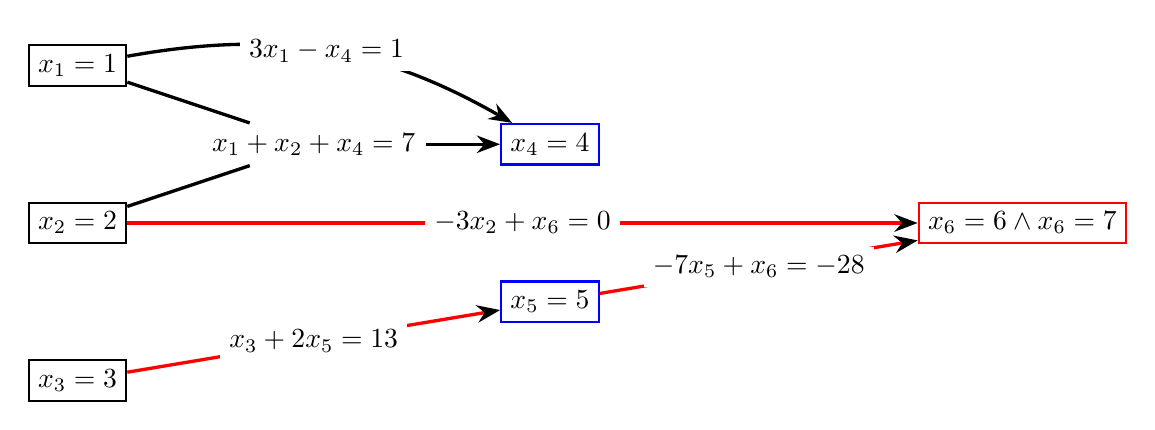
\begin{tikzpicture}
        \begin{scope}[every node/.style={rectangle,thick,draw}]
            \node (1) at (0,4) {$x_1 = 1$};
            \node[shape=rectangle,draw=none] (a) at (3,3) {$x_1 + x_2 + x_4 = 7$};
            \node (2) at (0,2) {$x_2 = 2$};
            \node (3) at (0,0) {$x_3 = 3$};
            \node[shape=rectangle,draw=blue] (4) at (6,3) {$x_4 = 4$};
            \node[shape=rectangle,draw=blue] (5) at (6,1) {$x_5 = 5$};
            \node[draw=red] (6) at (12,2) {$x_6 = 6 \land x_6 = 7$};
        \end{scope}

        \begin{scope}[>={Stealth[black]},
            every node/.style={fill=white,rectangle},
            every edge/.style={draw=black,very thick}]
            \path [-] (1) edge (a);
            \path [-] (2) edge (a);
            \path [->] (a) edge (4);
            \path [->] (1) edge[bend left=20] node {$3x_1 -  x_4 = 1$} (4);
            \path [->] (3) edge[draw=red] node {$x_3 + 2x_5 = 13$} (5);
            \path [->] (2) edge[draw=red] node {$-3x_2 + x_6 = 0$} (6);
            \path [->] (5) edge[draw=red] node {$-7x_5 + x_6 = -28$} (6);
        \end{scope}
    \end{tikzpicture}
    \caption{Example of a preprocessor graph. The given bounds (the nodes on the left) propagate using the constraints, inducing additional bounds (the blue nodes) that can be used to guide the solver.
        If a conflict is detected (red node), the edges responsible (red edges) are traced back to the origin to formulate an explanation to add to the SAT solver.
        In this case, the explanation adds the clause $(\neg l_1 \lor \neg l_2 \lor \neg l_3 \lor \neg l_4 \lor \neg l_5)$ where $l_1 \coloneqq x_2 = 2, l_2 \coloneqq x_3 = 3, l_3 \coloneqq -3x_2 + x_6 = 0, l_4 \coloneqq x_3 + 2x_5 = 13, l_5 \coloneqq -7x_5 + x_6 = -28$.
        Graphically, at least one of the red edges or the nodes from which they originate must be absent.}
    \label{dg:preprocessor}
\end{figure}

\subsection{LP solver}

\dlinear uses \soplex as its default LP solver.
It implements both the incremental precision boosting and the iterative refinement algorithms.
The user can choose between the two or even try a hybrid approach.
Because we are not interested in the optimal solution but in finding any solution, setting the objective function to $0$ to avoid pointless computations is a low-hanging fruit in terms of optimisation.
This is not the case in our implementations for reasons that will become clear in section~\ref{sec:strict-bounds}.

If a feasible solution is found, it means that the original formula is satisfiable, and the assignment is returned to the user.
Note that the solution's uniqueness is not guaranteed, so adding an artificial clause with the negation of the solution found will lead to another solution being found or the formula being declared unsatisfiable.
On the other hand, if the LP problem is infeasible, we can use the Farkas proof $y \in \bbbr^m$, corresponding to the last feasible solution of the dual problem before its unboundness or infeasibility was detected.
Given the initial $Ax \le b$ and $l \le x \le u$, we get an inequality $y^T A x \le y^T b$, which is infeasible over the local bounds, meaning that even setting $x_i$ to the bound that minimizes $y^T A$, the result will still be $y^T A x > y^T b$.
Collecting the constraints corresponding to the indexes where the Farkas proof is non-zero and the minimizing bounds makes it possible to determine a small infeasible subsystem of the original problem, albeit not necessarily an irreducible one, and use it to produce an explanation.

\subsection{Strict bounds}
\label{sec:strict-bounds}

To use out-of-the-box LP solvers as theory solvers, some adjustments in the formulation of the input may be required.
Strict inequalities are common in SMT formulae, but they are usually not supported by LP solvers. They would make the feasible region no longer closed, possibly making the search for the optimal solution pointless.
Other state-of-the-art SMT solver employing rational arithmetic within the theory solver~\footnote{z3 documentation: \url{https://z3prover.github.io/papers/z3internals.html\#sec-rational-linear-arithmetic}}, use a symbolic variable representing an infinitesimal parameter $\delta$ which enforces the inequality~\cite{ref:lra-dpll-t}.
Since our goal is to verify feasibility, we can reformulate the problem into an equi-feasible one while eliminating the strict inequalities at the cost of losing the original objective function.
We introduce a new variable called \textbf{strict variable}, $t$.
To simplify the notation, we only consider $<$ strict inequalities, but the same reasoning can be applied to $>$ since they can always be converted to $<$ by multiplying both sides by $-1$.
The same applies to $\ge$ and $=$, which can be converted to $\le$ as discussed in Section~\ref{sec:lp}.
Note that we are excluding \nqcs for now, as they will be discussed next.
Let $K$ indicate the set of indexes of strict inequality constraints ($<$) and with $J$ the set of indexes for all other constraints ($\le$).
Without loss of generality, assume that all the indices in $K$ are less than those in $J$ ($\max(J) < \min(K)$).
Using intuitive indexing over vector and matrix elements, start by replacing each strict inequality
\begin{align*}
    \sum_{i=1}^{n} a_{ki}x_{i} < b_k, \quad \forall k \in K
\end{align*}
with equivalent non-strict inequalities using the strict variable $t$:
\begin{align*}
    \sum_{i=1}^{n} a_{ki}x_{i} + t \le b_k, \quad \forall k \in K \\
    t > 0
\end{align*}
This change would only move the strict inequality problem to the bound on $t$.
However, it is possible to go a step further and relax the newly introduced bound by changing the objective function to maximize $t$.
The original problem we want to verify the feasibility of
\begin{equation}
    \label{eq:lp-original}
    \begin{split}
        \text{Maximize }   \quad & 0                                                          \\
        \text{subject to } \quad & \sum_{i=1}^{n} a_{ji}x_{i} \le b_j,  \quad \forall j \in J \\
        \quad                    & \sum_{i=1}^{n} a_{ki}x_{i} < b_k,   \quad \forall k \in K  \\
        & l_i \le x_i \le u_i,  \quad i \in \{1, 2, \ldots, n\}
    \end{split}
\end{equation}
can be relaxed to
\begin{equation}
    \label{eq:lp-relaxed}
    \begin{split}
        \text{Maximize }   \quad & t                                                             \\
        \text{subject to } \quad & \sum_{i=1}^{n} a_{ji}x_{i} \le b_j, \quad \forall j \in J     \\
        \quad                    & \sum_{i=1}^{n} a_{ki}x_{i} + t \le b_k, \quad \forall k \in K \\
        & l_i \le x_i \le u_i,  \quad i \in \{1, 2, \ldots, n\},        \\
        & t \ge 0
    \end{split}
\end{equation}

\begin{theorem}
    \label{thm:lp-relaxed}
    The original problem \eqref{eq:lp-original} is feasible if and only if the relaxed problem \eqref{eq:lp-relaxed} is feasible and there exists a solution that satisfies its constraints and for which the objective value is strictly greater than $0$.
\end{theorem}

\subsection{Not equal to constraints}

A more significant challenge is represented by \textit{not equal to} ($\ne$) constraints (\nqcs for short).
Let $D$ be the set of indexes of the \nqcs.
Again, without loss of generality, assume that all the indices in $D$ are greater than those in $K$ ($\max(K) < \min(D)$).
The extended relaxed problem is defined as
\begin{equation}
    \label{eq:lp-extended}
    \begin{split}
        \text{Maximize }   \quad & t                                                             \\
        \text{subject to } \quad & \sum_{i=1}^{n} a_{ji}x_{i} \le b_j, \quad \forall j \in J     \\
        \quad                    & \sum_{i=1}^{n} a_{ki}x_{i} + t \le b_k, \quad \forall k \in K \\
        \quad                    & \sum_{i=1}^{n} a_{di}x_{i} + t \le b_d, \quad \forall d \in D \\
        & l_i \le x_i \le u_i,  \quad i \in \{1, 2, \ldots, n\}         \\
        & t \ge 0
    \end{split}
\end{equation}

Two strict inequalities are needed to check whether the constraint is satisfied.
Since checking both simultaneously with an OR conjunction is impossible, the original problem must be split into two subproblems.
Hence, given $|D|$ \nqcs, $2^{|D|}$ problems must be solved (Eq.~\ref{eq:nq}).
\begin{equation}
    \label{eq:nq}
    \begin{gathered}
        \begin{cases}
            A_{1 \dots |J|} x \le b_{1 \dots |J| - 1}                 \\
            A_{|J| + 1\dots |J| + |K|} x < b_{|J| + 1\dots |J| + |K|} \\
            A_{|J| + |K| + 1} x \ne b_{|J| + |K| + 1}                 \\
            A_{|J| + |K| + 2} x \ne b_{|J| + |K| + 2}                 \\
        \end{cases}
        \\
        \text{will be split into}
        \\
        \begin{pmatrix}
            \begin{cases}
                A_{1 \dots |J|} x \le b_{1 \dots |J| - 1}                 \\
                A_{|J| + 1\dots |J| + |K|} x < b_{|J| + 1\dots |J| + |K|} \\
                A_{|J| + |K| + 1} x < b_{|J| + |K| + 1}                   \\
                A_{|J| + |K| + 2} x < b_{|J| + |K| + 2}
            \end{cases}
             &
            \begin{cases}
                A_{1 \dots |J|} x \le b_{1 \dots |J| - 1}                 \\
                A_{|J| + 1\dots |J| + |K|} x < b_{|J| + 1\dots |J| + |K|} \\
                A_{|J| + |K| + 1} x < b_{|J| + |K| + 1}                   \\
                A_{|J| + |K| + 2} x > b_{|J| + |K| + 2}
            \end{cases}
            \\
            \begin{cases}
                A_{1 \dots |J|} x \le b_{1 \dots |J| - 1}                 \\
                A_{|J| + 1\dots |J| + |K|} x < b_{|J| + 1\dots |J| + |K|} \\
                A_{|J| + |K| + 1} x > b_{|J| + |K| + 1}                   \\
                A_{|J| + |K| + 2} x < b_{|J| + |K| + 2}
            \end{cases}
             &
            \begin{cases}
                A_{1 \dots |J|} x \le b_{1 \dots |J| - 1}                 \\
                A_{|J| + 1\dots |J| + |K|} x < b_{|J| + 1\dots |J| + |K|} \\
                A_{|J| + |K| + 1} x > b_{|J| + |K| + 1}                   \\
                A_{|J| + |K| + 2} x > b_{|J| + |K| + 2}
            \end{cases}
        \end{pmatrix}
    \end{gathered}
\end{equation}
\eqcaption{Splitting an LP problem with 2 \nqcs into 4 subproblems. Note that the \nqcs appear in $4$ configurations: $\{<, <\}, \{<, >\}, \{>, <\}, \{>, >\}$.}

If any of the subproblems is feasible, then it is possible to conclude that the original problem is feasible.
On the other hand, in the worst case, all $2^{|D|}$ problems must be solved to prove infeasibility.
Some smarter heuristics can improve the average performance of the solver.
For instance, there is no need to continue solving subproblems if none of the \nqcs are involved in the infeasibility.
Furthermore, if only precisely one of them appears in the explanation, we can skip all other subproblems where it appears with the same sense, for they will surely be infeasible, too.
Also, we often only need to explore part of the tree to determine infeasibility.
If we find a subset of the \nqc that makes the problem infeasible on its own, we can immediately terminate the exploration.
We can obtain this early termination by enumerating the number of times a unique configuration of such a subset is solved.
If that number is equal to $2^{|T|}$, where $T$ is the set of indexes of the \nqcs in the subset, we can return an infeasibility explanation obtained by merging all the explanations produced by the subproblems that were enumerated.
Lastly, it is possible to \textit{hot start} the solver by starting in a configuration close to the one that caused the last infeasibility.

\subsection{Theory solver algorithm}

Let $\text{LpSolve}$ be a routine that, given a generic LP problem and the set of indexes corresponding to the senses of the constraints ($\le, <, \ne$), solves the extended relaxed problem (Eq. \eqref{eq:lp-extended}) and returns the set of indexes of infeasible constraints if there are any or an empty set otherwise.
To simplify the algorithm, only the essential heuristics are included in the pseudocode.
Keep in mind that $\odot$ represents an element-wise multiplication between two vectors or a vector and a scalar, with the scalar repeated to match the size of the vector.
\begin{algorithm}
    \caption{SMT adapted LP solver}\label{alg:theory-solver}
    \begin{algorithmic}
        \Require $A \in \bbbr^{(|J| + |K| + |D|) \times n}, b \in \bbbr^{|J| + |K| + |D|}, l \in \bbbr^n, u \in \bbbr^n$ \\
        \qquad as defined in Section~\ref{sec:lp} over the extended relaxed problem~\eqref{eq:lp-extended}
        \Require $J, K, D$ as defined in this Section \\
        \qquad note that $\max(J) < \min(K) \le \max(K) < \min(D)$
        \Ensure Set of indexes of infeasible constraints $E$ or $\emptyset$
        \State $E \gets \text{LpSolve}(A, b, l, u, J, K, \emptyset)$ \Comment{Solve the LP problem without $\ne$ constraints}
        \If{$E \ne \emptyset$}
        \State \Return $E$
        \EndIf
        \For {$s \in \text{ all non empty subsets of } D$}
        \State $V_s \gets \emptyset$
        \State $E_s \gets \emptyset$
        \EndFor
        \State $c \gets 0$ \Comment{Initialize the binary counter}
        \While{$c \le 2^{|D|}$}
        \State Let $C \in \{-1, 1\}^{|D|}$ be the binary representation of $c$ with $0$ replaced by $1$
        \State $C' \in \{-1, 1\}^{|J|+|K|+|D|} \gets \begin{bmatrix} 1^{|J|} & 1^{|K|} & C\end{bmatrix}$
        \State $A' \gets \begin{bmatrix}A_1 \odot C'_1 \\ \vdots \\ A_{|J|+|K|+|D|} \odot C'_{|J|+|K|+|D|}\end{bmatrix}$
        \State $E \gets \text{LpSolve}(A', b \odot C', l, u, J, K, D)$
        \If{$E = \emptyset$} \Comment{At least one subproblem is feasible}
        \State \Return $\emptyset$
        \EndIf
        \State $T \gets E \cap D$
        \State $l \gets (C'_{|J| + |K| + t}) \quad \forall t \in T$ % I want to construct a vector where each element is defined by the corresponding element in C' if the index is in T
        \If{$l \in V_T$} \Comment{Avoid adding redundant explanations for the same infeasibility}
        \State \textbf{Continue}
        \EndIf
        \State $V_T \gets V_T \cup \{l\}$
        \State $E_T \gets E_T \cup E$
        \If{$|V_T| = 2^{|T|}$} \Comment{Having explored it fully, a subset of the $\ne$ constraints is infeasible}
        \State \Return $E_T$
        \EndIf
        \State $c \gets c + 1$
        \EndWhile
        \State \Return $E$
    \end{algorithmic}
\end{algorithm}

% ---- Delta-completeness ----
\section{delta-completeness}
\label{sec:delta-completeness}

\dlinear offers the option to use delta-completeness.

% Taken from Martin's thesis
\begin{definition}
    If $\varphi$ is a Boolean formula in which every atomic formula is of one the forms $t(x) \bowtie 0$ is an arbitrary term, then the $\delta$-weakening of $\varphi$ for any $\delta > 0$, denoted $\varphi^{-\delta}$, is the formula obtained by replacing every constraint $t(x) = 0$ with $|t(x)| \le \delta$, $t(x) \le 0$ with $t(x) \le \delta$ relaxing the strict inequalities from $t(x) < 0$ to $t(x) \le \delta$ and removing all \nqcs.
\end{definition}
Denoting with $J'$ the set of indexes of those that were equality constraints in $\varphi$ and with $K'$ the one with every other constraint except for \nqcs, then $\varphi^{-\delta}$ can be written as
\begin{equation*}
    \varphi^{-\delta} = \bigwedge_{j \in J'} |t_j(x)| \le \delta \wedge \bigwedge_{k \in K'} t_k(x) \le \delta
\end{equation*}
with the corresponding LP problem being
\begin{equation}
    \label{eq:delta-lp}
    \begin{split}
        \text{Maximize }   \quad & 0                                                                                \\
        \text{subject to } \quad & \left|\sum_{i=1}^{n} a_{ji}x_{i}\right| \le b_j + \delta, \quad \forall j \in J' \\
        \quad                    & \sum_{i=1}^{n} a_{ki}x_{i} \le b_k + \delta, \quad \forall k \in K'              \\
        \quad                    & l_i - \delta \le x_i \le u_i + \delta,  \quad i \in \{1, 2, \ldots, n\}
    \end{split}
\end{equation}
\begin{definition}
    A $\delta$-complete decision procedure for satisfiability over a class of formulae $F$ is an algorithm that, if provided as input any formula $\varphi \in F$, terminates and outputs (non-deterministically) exactly one of the following symbols:
    \begin{enumerate}
        \item unsat only if $\varphi$ is unsatisfiable
        \item $\delta$-sat only if $\varphi^{-\delta}$ (the $\delta$-weakening of $\varphi$) is satisfiable
    \end{enumerate}
\end{definition}
Note that such a procedure is non-deterministic because both conditions can simultaneously be true.
Furthermore, any complete method is, by definition, trivially $\delta$-complete.
The advantage of this approach is that the LP solver can stop refining the solution as soon as the arbitrary precision $\delta$, indicated by the user, is reached, possibly saving computation time, especially for numerically challenging instances.
Leaving out the \nqcs also removes the potentially most computationally expensive part of the problem, as discussed in Section~\ref{sec:lra-theory-solver}.
Whether this tradeoff between speed and completeness is acceptable is up to the user to decide.

To implement delta-completeness in \dlinear, the user can set the $\delta$ parameter to a positive value, then given to the LP solver.
The precision boosting or iterative refinement algorithms can stop once the desired precision has been reached, returning the solution found at that point.

Let $\text{DeltaLpSolve}$ be a routine that, given a generic LP problem and the set of indexes corresponding to the senses of the original constraints ($=, \le$), solves the delta weakened problem (Eq. \eqref{eq:delta-lp}) and returns the set of indexes of infeasible constraints if there are any or an empty set otherwise.
We can define the delta-complete theory solver algorithm as in Algorithm~\ref{alg:delta-theory-solver}.

% Inspired by Martin's thesis. I'm not sure this contributes anything useful to the explanation
\begin{algorithm}
    \caption{SMT adapted delta complete LP solver}\label{alg:delta-theory-solver}
    \begin{algorithmic}
        \Require $A \in \bbbr^{(|J'| + |K'|) \times n}, b \in \bbbr^{|J'| + |K'|}, l \in \bbbr^n, u \in \bbbr^n$ \\
        \qquad as defined in Section~\ref{sec:lp} over the delta weakened problem~\eqref{eq:delta-lp}
        \Require $J', K'$ as defined in this Section
        \Require $\delta > 0$
        \Ensure Set of indexes of infeasible constraints $E$ or $\emptyset$
        \State $E \gets \text{DeltaLpSolve}(A, b, l, u, J', K', \delta)$ \Comment{Solve the LP problem with $\delta$-weakened constraints}
        \State \Return $E$
    \end{algorithmic}
\end{algorithm}


\section{Neural network verification}
\label{sec:nn-verification}

\dlinear can be used to verify neural networks that utilize ReLU activation functions.
Given a description of the network that utilizes the Open Neural Network Exchange (ONNX) format~\footnote{\url{https://onnx.ai/index.html}}, the acyclic graph that describes all the layers of the network gets parsed, from inputs to outputs (\autoref{fig:netron}).

\begin{wrapfigure}{r}{.25\textwidth} %this figure will be at the right
    \centering
    \begin{adjustbox}{width=.1\textwidth,center}
        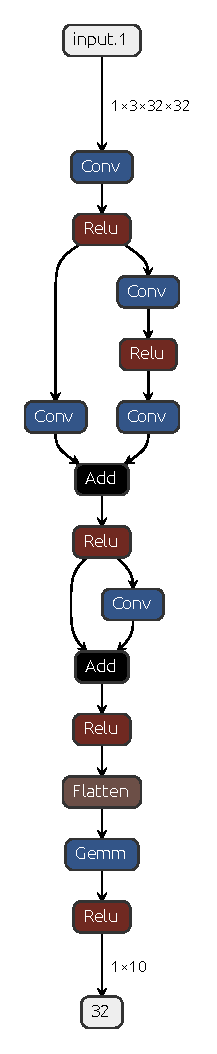
\includegraphics[width=.1\textwidth]{img/netron.eps}
    \end{adjustbox}
    \caption{ONNX visualization by Netron}\label{fig:netron}
\end{wrapfigure}

Exploring the graph, most of the network layers are converted into linear constraints that can be handled by the \dlinear's SMT solver functionalities.
Upon encountering a piecewise linear activation function, we introduce a fresh variable $y'$ and as many linear constraints as there are cases in the function by encoding an equality between the fresh variable and the output of the activation function.
All the linear constraints are then added to the set of assertions in a "at most one" encoding.
The fresh variable replaces the corresponding linear constraint for all the dependent nodes of the graph from that point on.
For instance, the ReLU activation function can be represented as

$$
    y' = \begin{cases}
        x & \text{if } x \ge 0 \\
        0 & \text{otherwise}
    \end{cases}
$$

Given the two formulae $A \coloneqq (y' = x), B \coloneqq (y' = 0)$, the clauses $(A \lor B) \land (\neg A \lor \neg B)$ are added to the set of assertions.

Even limiting ourselves to the common ReLU layer, the number of subproblems grows exponentially, making the verification process computationally intractable even for medium sized networks.
To mitigate this issue, we can try to exploit the structure of the problem.
The bound propagation mentioned in Section~\ref{sec:preprocessing} is adapted to iteratively tighten the bounds of the output of each layer.
In the best case, the newly found bounds can uniquely indicate the only branch a piecewise function can take, reducing the search space.

The piecewise functions are encoded as a Sum of Infeasibilities (SoI), which becomes the objective function to minimize while the other linear expression create the constraints the problem is subject to.
% TODO


% ---- Benchmarks ----
\section{Benchmarks}
\label{sec:benchmarks}
\subsection*{Specifications}

We compared \dlinear with the following state-of-the-art tools: cvc5~\cite{ref:cvc5} (version 1.0.8), Z3~\cite{ref:z3} (version 4.12.2).
The benchmarking suite has been run on a CentOS machine with 2 Intel Xeon E5-2699 v4 processors @ 2.2 GHz, 22 cores, 55 MB cache, and a memory limit of 2.9GB (DDR4 RDIMMs).
The timeout was set to 6 hours.

\subsection*{Result}

TODO

\begin{credits}
    \subsubsection{\ackname} This study was funded by EPSRC
\end{credits}

% ---- Bibliography ----
\bibliographystyle{splncs04}
\bibliography{resources}

% ---- Appendices ----
% \begin{appendices}
%     Proof of~\autoref{thm:lp-relaxed}.
%     \chapter{Proof}
%     \begin{proof}
%         Without loss of generality, assume that both linear programming problems are in standard form.
%         Let $J$ be the set of indexes of strict inequality constraints, and $K$ be the set of indexes for all other constraints.
%         \\
%         \framedtext{\eqref{eq:lp-original} feasible $\implies$ \eqref{eq:lp-relaxed} feasible $\land$  \eqref{eq:lp-relaxed} objective value $> 0$} \\

%         If the original problem is feasible, then there exists a solution, a set of values to be assigned to the decision variables $x_1, x_2, \ldots, x_n$, that satisfies all the constraints.
%         For the strict inequality constraints to be satisfied, it means that there exists a value $\delta_j > 0, \quad j \in J$ such that
%         \begin{align*}
%             \sum_{i=1}^{n} a_{ji}x_{i} + \delta_j = b_j, \quad \forall j \in J
%         \end{align*}
%         Let $\bar{t} = \min(\delta_j), \quad j \in J$.
%         The expression becomes
%         \begin{align*}
%             \sum_{i=1}^{n} a_{ji}x_{i} + \bar{t} \le b_j, \quad \forall j \in J \\
%             \bar{t} > 0
%         \end{align*}
%         which is the formulation of the previously strict constraints used in the relaxed problem.
%         All other constraints have been left unchanged, therefore the solution to the original problem can be used to satisfy the constraints of the relaxed problem by also setting $t = \bar{t}$ which is greater than $0$.
%         Hence, the objective value of the relaxed problem is $> 0$.
%         \\
%         \framedtext{\eqref{eq:lp-relaxed} feasible $\land$  \eqref{eq:lp-relaxed} objective value $> 0$ $\implies$ \eqref{eq:lp-original} feasible} \\

%         The solution to the relaxed problem already satisfies all the non-strict constraints of the original problem.
%         The objective value is greater than $0$; therefore, $t > 0$.
%         Since all relaxed constraints in the form
%         \begin{align*}
%             \sum_{i=1}^{n} a_{ji}x_{i} + t \le b_j, \quad \forall j \in J \\
%             t > 0
%         \end{align*}
%         are satisfied the original strict inequality constraints
%         \begin{align*}
%             \sum_{i=1}^{n} a_{ji}x_{i} < b_j, \quad \forall j \in J
%         \end{align*}
%         are also satisfied.
%         Hence, the original problem is feasible.
%     \end{proof}

% \end{appendices}

\end{document}
